\documentclass{exam}
\usepackage{graphicx} 

% Enable solutions and customize solution name
\printanswers
\pointpoints{poäng}{poäng}
\pointformat{\textbf{\thepoints}}
\renewcommand{\solutiontitle}{\noindent\textbf{Lösningsförslag:}\enspace}

% Format Header and footer
\pagestyle{headandfoot}
\header{\footnotesize Klass:\\Namn:}{\Large\textbf{Fysiologi - Facit}\\\medskip\small Gastro-intestinala, Respirationen, Cirkulationen och Exkretionen}{\footnotesize BIOBIO02 - 2025\\Viktor Arohlén}
\headrule
\footrule
\setlength{\columnsep}{0.25cm}
\footer{}{Sida \thepage}{}

\begin{document}
\section*{Instruktioner}
Provet består av två delar \\
    - Grundläggande frågor, svara kortfattat (\textit{14 poäng})\\
    - Fördjupande frågor, svara mer omfattande (\textit{10 poäng} + 2 bonuspoäng)

\subsection*{Poäng}
Antalet poäng är markerat för varje fråga. Totalt \textbf{12 frågor} och \textbf{24 poäng}.\\ \textit{För godkänt resultat krävs 10 poäng.}

\vspace{5mm} %5mm vertical space
\begin{center}
\fbox{\fbox{\parbox{6in}{\centering
\textbf{Grundläggande frågor}: svara kortfattat (\textbf{14 poäng})
}}}
\end{center}
\begin{questions}

\question I vilken ordning passerar blodet genom följande strukturer? (\textbf{2 poäng})

\begin{itemize}
  \item Vänster förmak
  \item Lungartär
  \item Aorta
  \item Lungven
  \item Vänster kammare
  \item Kapillär
  \item Ven
\end{itemize}

\begin{solution}
Korrekt ordning:
1. Ven → 
2. Vänster förmak → 
3. Vänster kammare → 
4. Aorta → 
5. Kapillär → 
6. Lungartär → 
7. Lungven

Detta representerar blodets väg genom det systemiska och pulmonära kretsloppet.
\end{solution}

\vspace{5mm}

\question Beskriv två \textbf{vävnadstyper} och ge exempel på i vilka organ vi hittar dem. (\textbf{2 poäng})
\begin{solution}
Två exempel på vävnadstyper:

1. \textbf{Epitelväv}:
   - Täcker kroppens ytor och organ
   - Finns i huden, matsmältningskanalen och luftvägarna
   - Skyddande funktion och specialiserad för absorption/sekretion

2. \textbf{Muskelväv}:
   - Finns i tre former: skelettmuskulatur, glatt muskulatur och hjärtmuskulatur
   - Skelettmuskulatur: i muskler kopplade till skelettet
   - Glatt muskulatur: i blodkärl och matsmältningskanal
   - Hjärtmuskulatur: endast i hjärtat
\end{solution}

\question Vad av följande är \textbf{inte} en vitamin eller mineral? (\textbf{1 poäng})
\begin{checkboxes}
    \choice Biotin
    \choice Zink
    \choice Askorbinsyra
    \correctchoice Omega-3
\end{checkboxes}

\begin{solution}
Omega-3 är en fettsyra, inte en vitamin eller mineral. De andra alternativen är:
- Biotin (vitamin B7)
- Zink (mineral)
- Askorbinsyra (vitamin C)
\end{solution}

\question Vad av följande är \textbf{stämmer} för ett djur som lever i sötvatten? (\textbf{1 poäng})
\begin{checkboxes}
    \choice De måste ta upp mer salt från omgivningen
    \choice De har en koncentrerad urin för att behålla saltbalansen
    \correctchoice De har en utspädd urin för att behålla saltbalansen
    \choice Deras omgivning har högre saltkoncentration än dem
\end{checkboxes}

\begin{solution}
Djur i sötvatten har högre saltkoncentration än omgivningen (hypoton miljö). Vatten strömmar därför in i kroppen genom osmos. För att kompensera producerar de stora mängder utspädd urin för att bli av med överflödigt vatten och behålla saltbalansen.
\end{solution}

\question Beskriv för- och nackdelar för organismer som är \textbf{herbivorer} (växtätare) (\textbf{2 poäng})
\begin{solution}
\textbf{Fördelar:}
- Riklig tillgång till föda
- Mindre energikrävande att jaga/fånga föda
- Ofta lättare att hitta föda året runt
- Mindre risk att skadas vid födosök

\textbf{Nackdelar:}
- Växtmaterial är svårsmält och näringsfattigt
- Kräver specialiserad matsmältning (långa tarmar, specialiserade enzymer)
- Behöver äta stora mängder för att få tillräckligt med näring
- Ofta beroende av symbiotiska bakterier för att bryta ned cellulosa
\end{solution}

\question Vad av följande \textbf{reglerer} den \textit{automatiska} andningen i första hand? (\textbf{1 poäng})
\begin{checkboxes}
    \choice Syrekoncentrationen
    \choice Hjärtats retledningssystem
    \correctchoice Blodets pH
    \choice Blodtrycket i njuren
\end{checkboxes}

\begin{solution}
Andningscentrum i hjärnstammen reglerar främst andningen baserat på blodets pH-värde, vilket påverkas av koldioxidhalten. När CO₂ stiger sjunker pH, vilket stimulerar ökad andning för att vädra ut CO₂ och normalisera pH.
\end{solution}

\question Vilka \textit{strukturella} skillnader finns det mellan en \textbf{ven} och en \textbf{artär}? (\textbf{2 poäng})
\begin{solution}
Strukturella skillnader mellan vener och artärer:

\textbf{Artärer:}
- Tjockare, mer elastisk vägg
- Mer muskelvävnad i väggen
- Mindre lumen (inre diameter)
- Inga klaffar (förutom i hjärtat)

\textbf{Vener:}
- Tunnare vägg
- Mindre muskelvävnad
- Större lumen
- Har klaffar för att förhindra återflöde
\end{solution}

\question Vad av följande \textbf{stämmer} den \textit{automatiska} andningen i första hand? (\textbf{1 poäng})
\begin{checkboxes}
    \choice Syrekoncentrationen
    \choice Hjärtats retledningssystem
    \correctchoice Blodets pH
    \choice Blodtrycket i njuren
\end{checkboxes}

\begin{solution}
Samma som tidigare fråga - andningen regleras primärt av blodets pH-värde genom koldioxidnivåer som detekteras av kemoreceptorer i hjärnstammen.
\end{solution}

\question Markera om följande påståenden är \textbf{sanna} eller \textbf{falska}: (\textbf{2 poäng})

\begin{oneparchoices}
    \choice Enzymet amylas bryter ner proteiner i tunntarmen. \hfill \textbf{Falskt}
    \vspace{2mm}
    \choice Njurarna filtrerar cirka 180 liter primärurin per dag. \hfill \textbf{Sant}
    \vspace{2mm}
    \choice Alveolerna i lungorna är omgivna av kapillärer. \hfill \textbf{Sant}
    \vspace{2mm}
    \choice Gallblåsan producerar enzymer som bryter ner fetter. \hfill \textbf{Falskt}
    \vspace{2mm}
    \choice Saltsyran i magsäcken är viktig för att aktivera enzymer. \hfill \textbf{Sant}
    \vspace{2mm}
    \choice Kolhydrater börjar brytas ned redan i munhålan. \hfill \textbf{Sant}
    \vspace{2mm}
    \choice Klaffarna i venerna förhindrar att blodet flödar bakåt. \hfill \textbf{Sant}
    \vspace{2mm}
    \choice Njuren är viktig för att reglera blodvolymen. \hfill \textbf{Sant}
\end{oneparchoices}

\begin{solution}
Förklaringar:
- Amylas bryter ner kolhydrater, inte proteiner
- 180L primärurin är korrekt, men det mesta återabsorberas
- Alveolerna är tätt omgivna av kapillärer för gasutbyte
- Gallblåsan lagrar galla från levern, producerar inte enzymer
- Saltsyra aktiverar pepsinogen till pepsin
- Amylas i saliven börjar bryta ner kolhydrater
- Venklaffar är essentiella för blodets återflöde till hjärtat
- Njuren reglerar blodvolym genom att justera vattenreabsorption
\end{solution}

\break

\vspace{5mm}
\begin{center}
\fbox{\fbox{\parbox{6in}{\centering
\textbf{Fördjupande frågor}: svara mer utförligt (\textbf{10 poäng} + 2 bonuspoäng)
}}}
\end{center}

\question
En person börjar springa ett maraton. Utifrån dina kunskaper, beskriv vad som händer i följande organsystem för att bibehålla homeostas under den fysiska ansträngningen? (\textbf{4 poäng})

\begin{solution}
\textbf{Respirationssystemet:}
- Ökad andningsfrekvens och djup
- Effektivare gasutbyte i alveolerna
- Ökad syretillförsel till arbetande muskler
- Ökad CO₂-eliminering för att motverka pH-sänkning

\textbf{Cirkulationssystemet:}
- Ökad hjärtfrekvens och slagvolym
- Omfördelning av blodflöde till arbetande muskler
- Vidgning av blodkärl i muskler (vasodilation)
- Ökad svettning för temperaturreglering

\textbf{Gastro-intestinala systemet:}
- Minskad aktivitet (blod omdirigeras)
- Ökad glukosanvändning från glykogenlager
- Ökad fettförbränning vid längre aktivitet
- Minskad matsmältningsaktivitet

\textbf{Utsöndringssystemet:}
- Minskad urinproduktion
- Ökad återabsorption av vatten
- Ökad svettproduktion
- Elektrolytbalans justeras för att kompensera för svettförluster
\end{solution}

\question
En rubbad homeostas är ofta \textbf{patologiskt}(sjukligt). Ge exempel på hur en sjukdom kan påverka homeostasen i något av de organsystem som diskuterats? (\textbf{2 poäng})

\begin{solution}
\textbf{Exempel: Diabetes typ 1}
- Påverkar flera organsystem genom brist på insulin:

\textbf{Primär effekt:}
- Oförmåga att reglera blodsocker
- Celler kan inte ta upp glukos effektivt
- Ökad nedbrytning av fett och protein

\textbf{Systemeffekter:}
1. Utsöndringssystemet:
   - Ökad urinproduktion
   - Uttorkning
   - Elektrolytobalans

2. Cirkulationssystemet:
   - Påverkad blodvolym
   - Risk för kärlskador

3. Gastro-intestinala systemet:
   - Förändrad metabolism
   - Störd näringsupptag
\end{solution}

\question Nedan ses ett EKG. Med bilden som hjälp besvara följande frågor: (\textbf{4 poäng})
\begin{figure}[h]
\centering
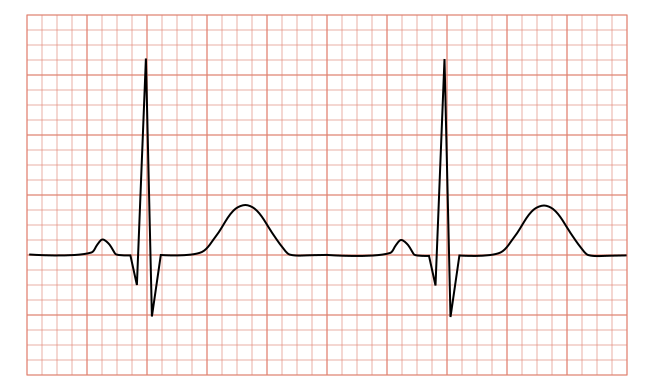
\includegraphics[width=0.5\textwidth]{EKG.png}
\end{figure}

\begin{solution}
\textbf{Vad visualiseras i ett EKG?}
- EKG visar hjärtats elektriska aktivitet över tid
- P-vågen: förmakens depolarisering
- QRS-komplexet: kamrarnas depolarisering
- T-vågen: kamrarnas repolarisering

\textbf{Vad sker i hjärtat:}
1. P-våg: förmaken kontraherar
2. QRS: kamrarna kontraherar
3. T-våg: kamrarna återgår till vilofas

\textbf{Användning för att upptäcka hjärtsjukdomar:}
- Arytmier: oregelbunden rytm eller onormal frekvens
- Hjärtinfarkt: ST-höjning eller Q-vågsförändringar
- Förmaksflimmer: oregelbunden förmaksaktivitet
- Grenblock: förändrat QRS-komplex
- Hypertrofi: ökad amplitud i vissa vågor
\end{solution}

\question \textbf{BONUS}: Beskriv något du lärt dig och tyckt varit extra intressant, men som inte var med på provet! (\textbf{2 bonuspoäng})
\begin{solution}
Detta är en öppen fråga där eleverna kan visa fördjupad förståelse och intresse för ämnet. Några exempel på bra svar:
- Detaljerad beskrivning av specifika sjukdomar och deras påverkan på kroppen
- Förklaring av komplexa feedback-system
- Kopplingar mellan olika organsystem
- Evolutionära anpassningar i olika organsystem
- Aktuell forskning inom fysiologi
\end{solution}

\end{questions}
\end{document}
